\documentclass[a4paper,12pt]{article}
\usepackage{xcolor}
\usepackage{amsmath,amsfonts,amssymb}
\usepackage{geometry}
\usepackage{fancyhdr}
\usepackage{graphicx}
\usepackage{titlesec}
\usepackage{tikz}
\usepackage{booktabs}
\usepackage{array}
\usetikzlibrary{shadows}
\usepackage{tcolorbox}
\usepackage{float}
\usepackage{lipsum}
\usepackage{mdframed}
\usepackage{pagecolor}
\usepackage{mathpazo}   % Palatino font (serif)
\usepackage{microtype}  % Better typography

% Page background color
\pagecolor{gray!10!white}

% Geometry settings
\geometry{margin=0.5in}
\pagestyle{fancy}
\fancyhf{}

% Fancy header and footer
\fancyhead[C]{\textbf{\color{blue!80}CS378 Lab-8}}
\fancyhead[R]{\color{blue!80}Saksham Rathi}
\fancyfoot[C]{\thepage}

% Custom Section Color and Format with Sans-serif font
\titleformat{\section}
{\sffamily\color{purple!90!black}\normalfont\Large\bfseries}
{\thesection}{1em}{}

% Custom subsection format
\titleformat{\subsection}
{\sffamily\color{cyan!80!black}\normalfont\large\bfseries}
{\thesubsection}{1em}{}

% Stylish Title with TikZ (Enhanced with gradient)
\newcommand{\cooltitle}[1]{%
  \begin{tikzpicture}
    \node[fill=blue!20,rounded corners=10pt,inner sep=12pt, drop shadow, top color=blue!50, bottom color=blue!30] (box)
    {\Huge \bfseries \color{black} #1};
  \end{tikzpicture}
}
\usepackage{float} % Add this package

\newenvironment{solution}[2][]{%
    \begin{mdframed}[linecolor=blue!70!black, linewidth=2pt, roundcorner=10pt, backgroundcolor=yellow!10!white, skipabove=12pt, skipbelow=12pt]%
        \textbf{\large #2}
        \par\noindent\rule{\textwidth}{0.4pt}
}{
    \end{mdframed}
}

% Document title
\title{\cooltitle{CS378 Lab-8}}
\author{{\bf Saksham Rathi} \\
\small Department of Computer Science, \\
Indian Institute of Technology Bombay \\
{\bf 22B1003}}
\date{}

\begin{document}
\maketitle
\begin{solution}{Result Plots}
    Here are the plots:
    \begin{figure}[H]
        \centering
        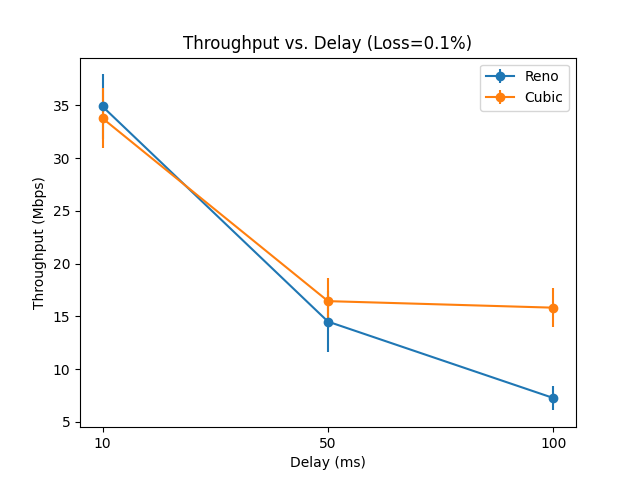
\includegraphics[width=0.8\textwidth]{throughput_vs_delay_loss_0.1.png}
        \caption{Throughput vs Delay for Loss  0.1\%}
    \end{figure}

    \begin{figure}[H]
        \centering
        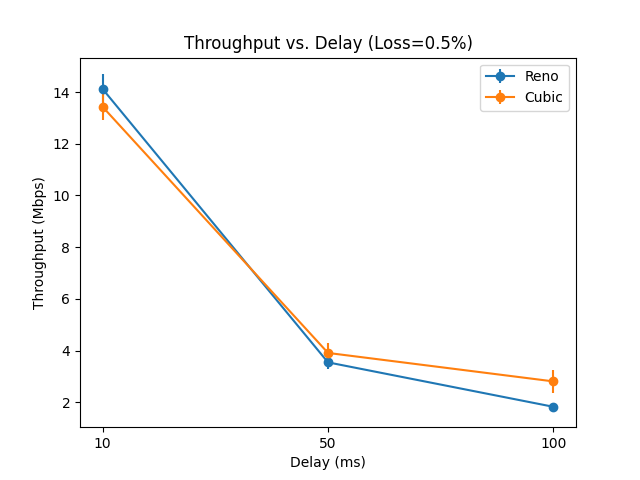
\includegraphics[width=0.8\textwidth]{throughput_vs_delay_loss_0.5.png}
        \caption{Throughput vs Delay for Loss  0.5\%}
    \end{figure}

    \begin{figure}[H]
        \centering
        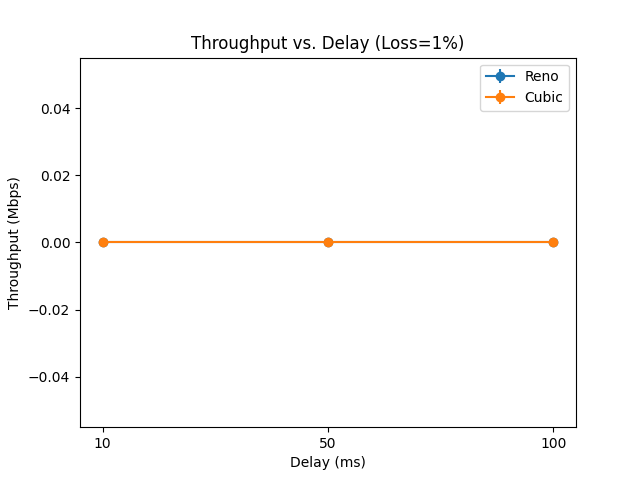
\includegraphics[width=0.8\textwidth]{throughput_vs_delay_loss_1.png}
        \caption{Throughput vs Delay for Loss  1.0\%}
    \end{figure}

    

    \begin{figure}[H]
        \centering
        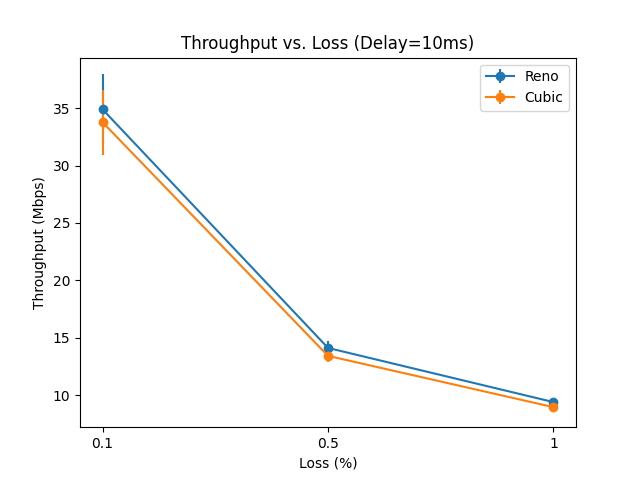
\includegraphics[width=0.8\textwidth]{throughput_vs_loss_delay_10ms.png}
        \caption{Throughput vs Loss for Delay 10ms}
    \end{figure}

    \begin{figure}[H]
        \centering
        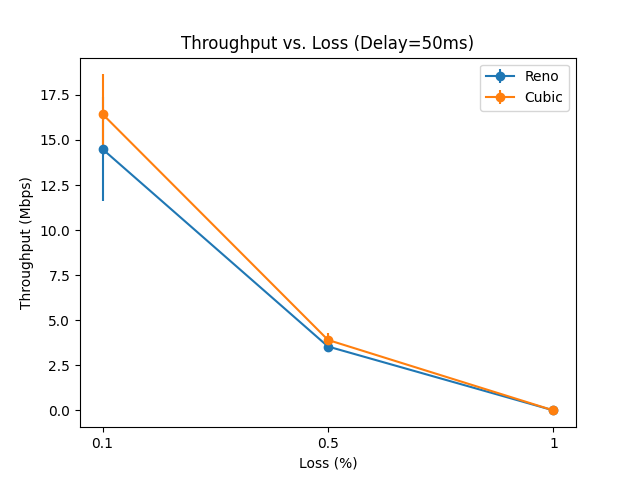
\includegraphics[width=0.8\textwidth]{throughput_vs_loss_delay_50ms.png}
        \caption{Throughput vs Loss for Delay 50ms}
    \end{figure}

    \begin{figure}[H]
        \centering
        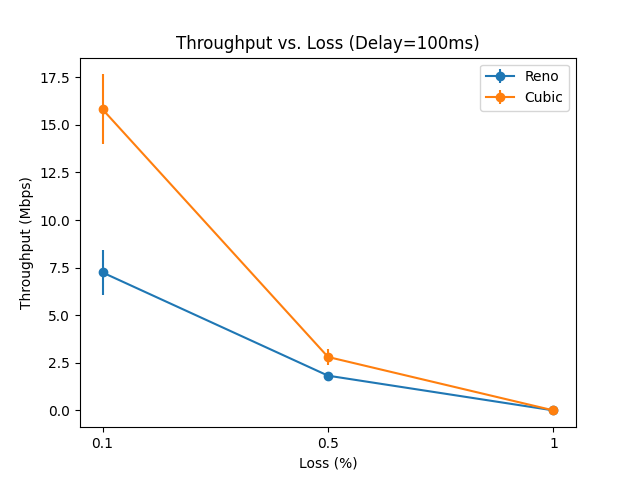
\includegraphics[width=0.8\textwidth]{throughput_vs_loss_delay_100ms.png}
        \caption{Throughput vs Loss for Delay 100ms}
    \end{figure}
\end{solution}

\begin{solution}{Observations}
    \begin{itemize}
        \item In all of the plots (and for all of the datapoints), the throughput from cubic is higher than that from reno. This is because cubic is more aggressive in increasing the congestion window size. Therefore it is able to send more packets in the same time (and a higher throughput is observed).
        \item The throughput decreases as the delay increases. This is because the packets take more time to reach the destination and the sender has to wait for the ACKs. This increases the RTT and hence the throughput decreases. This again confirms the theoretical result that throughput is inversely proportional to the RTT.
        \item The loss percentage field represents the rate at which packets are dropped. As the loss percentage increases, the throughput decreases. This is because the sender has to retransmit the packets that are lost. This increases the RTT and hence the throughput decreases. When the packet loss rate is 1\%, the throughput is really low because the sender has to retransmit almost all the packets.
    \end{itemize}
\end{solution}

\clearpage

\begin{solution}{Wireshark Plots}
    Here are the window scaling graphs from Wireshark:
    \begin{figure}[H]
        \centering
        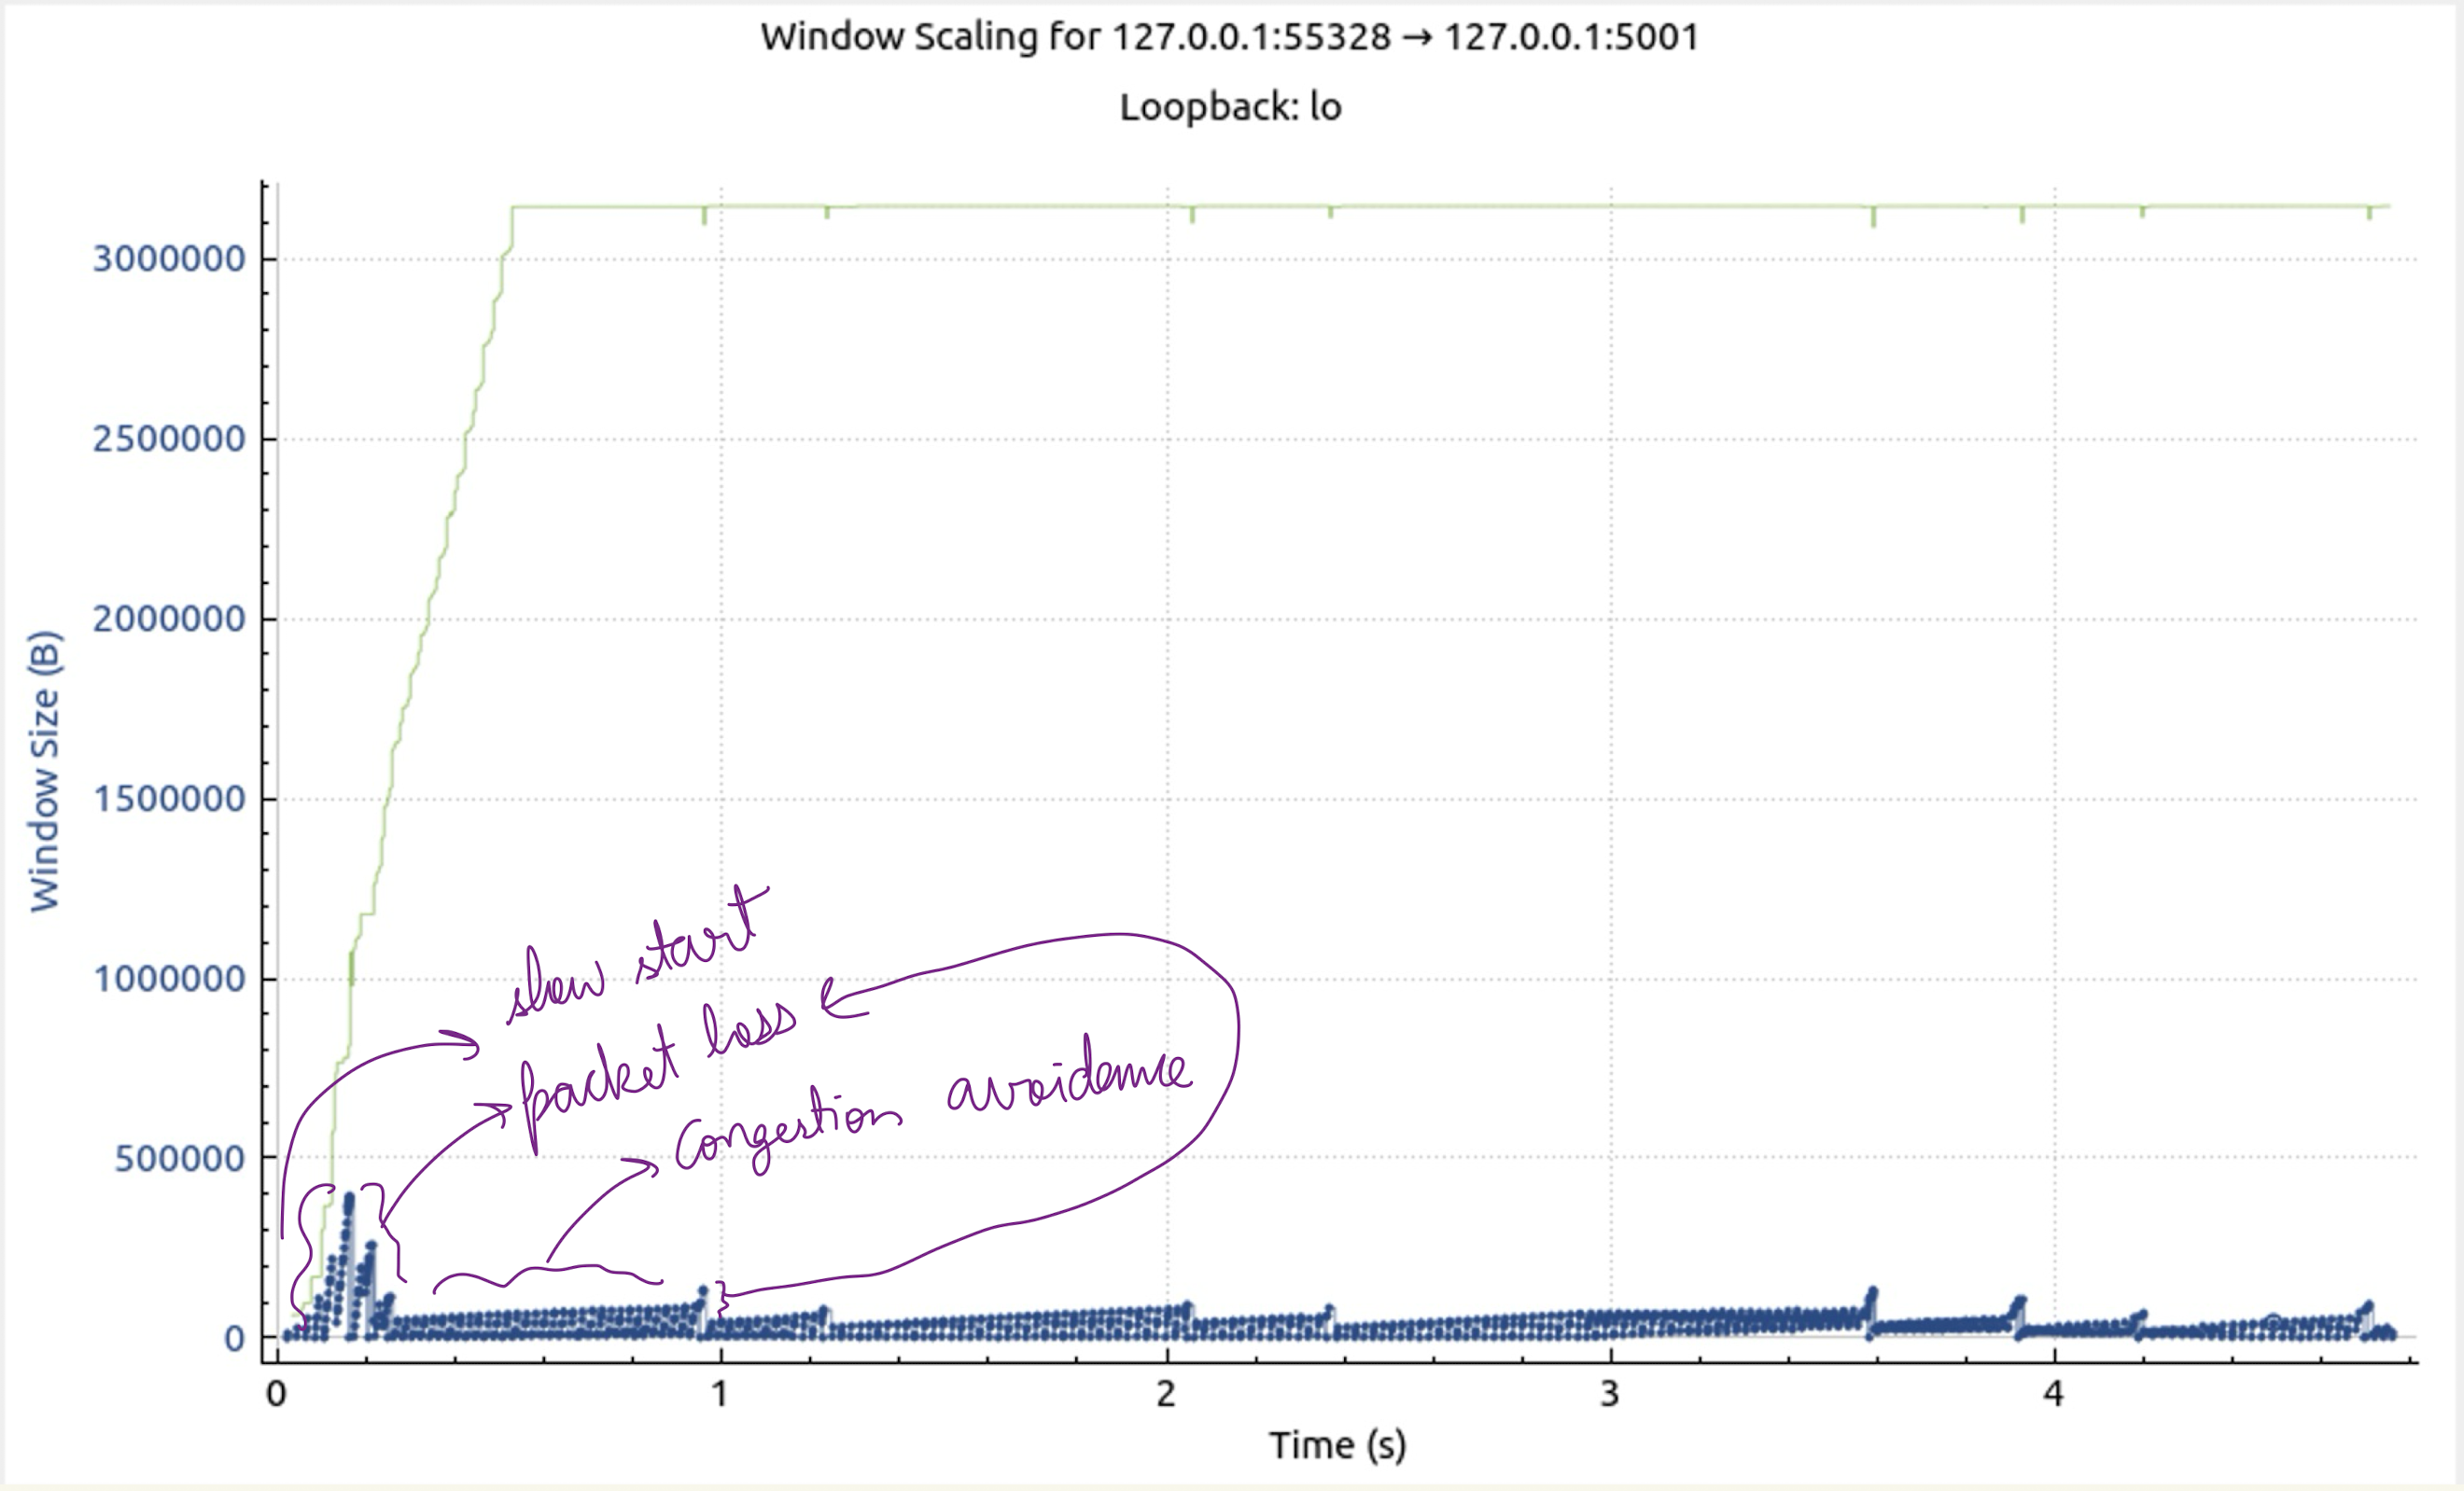
\includegraphics[width=0.8\textwidth]{reno-e1.png}
        \caption{Reno Window Scaling Graph for Delay=10ms and Loss=0.1\%}
    \end{figure}

    \begin{figure}[H]
        \centering
        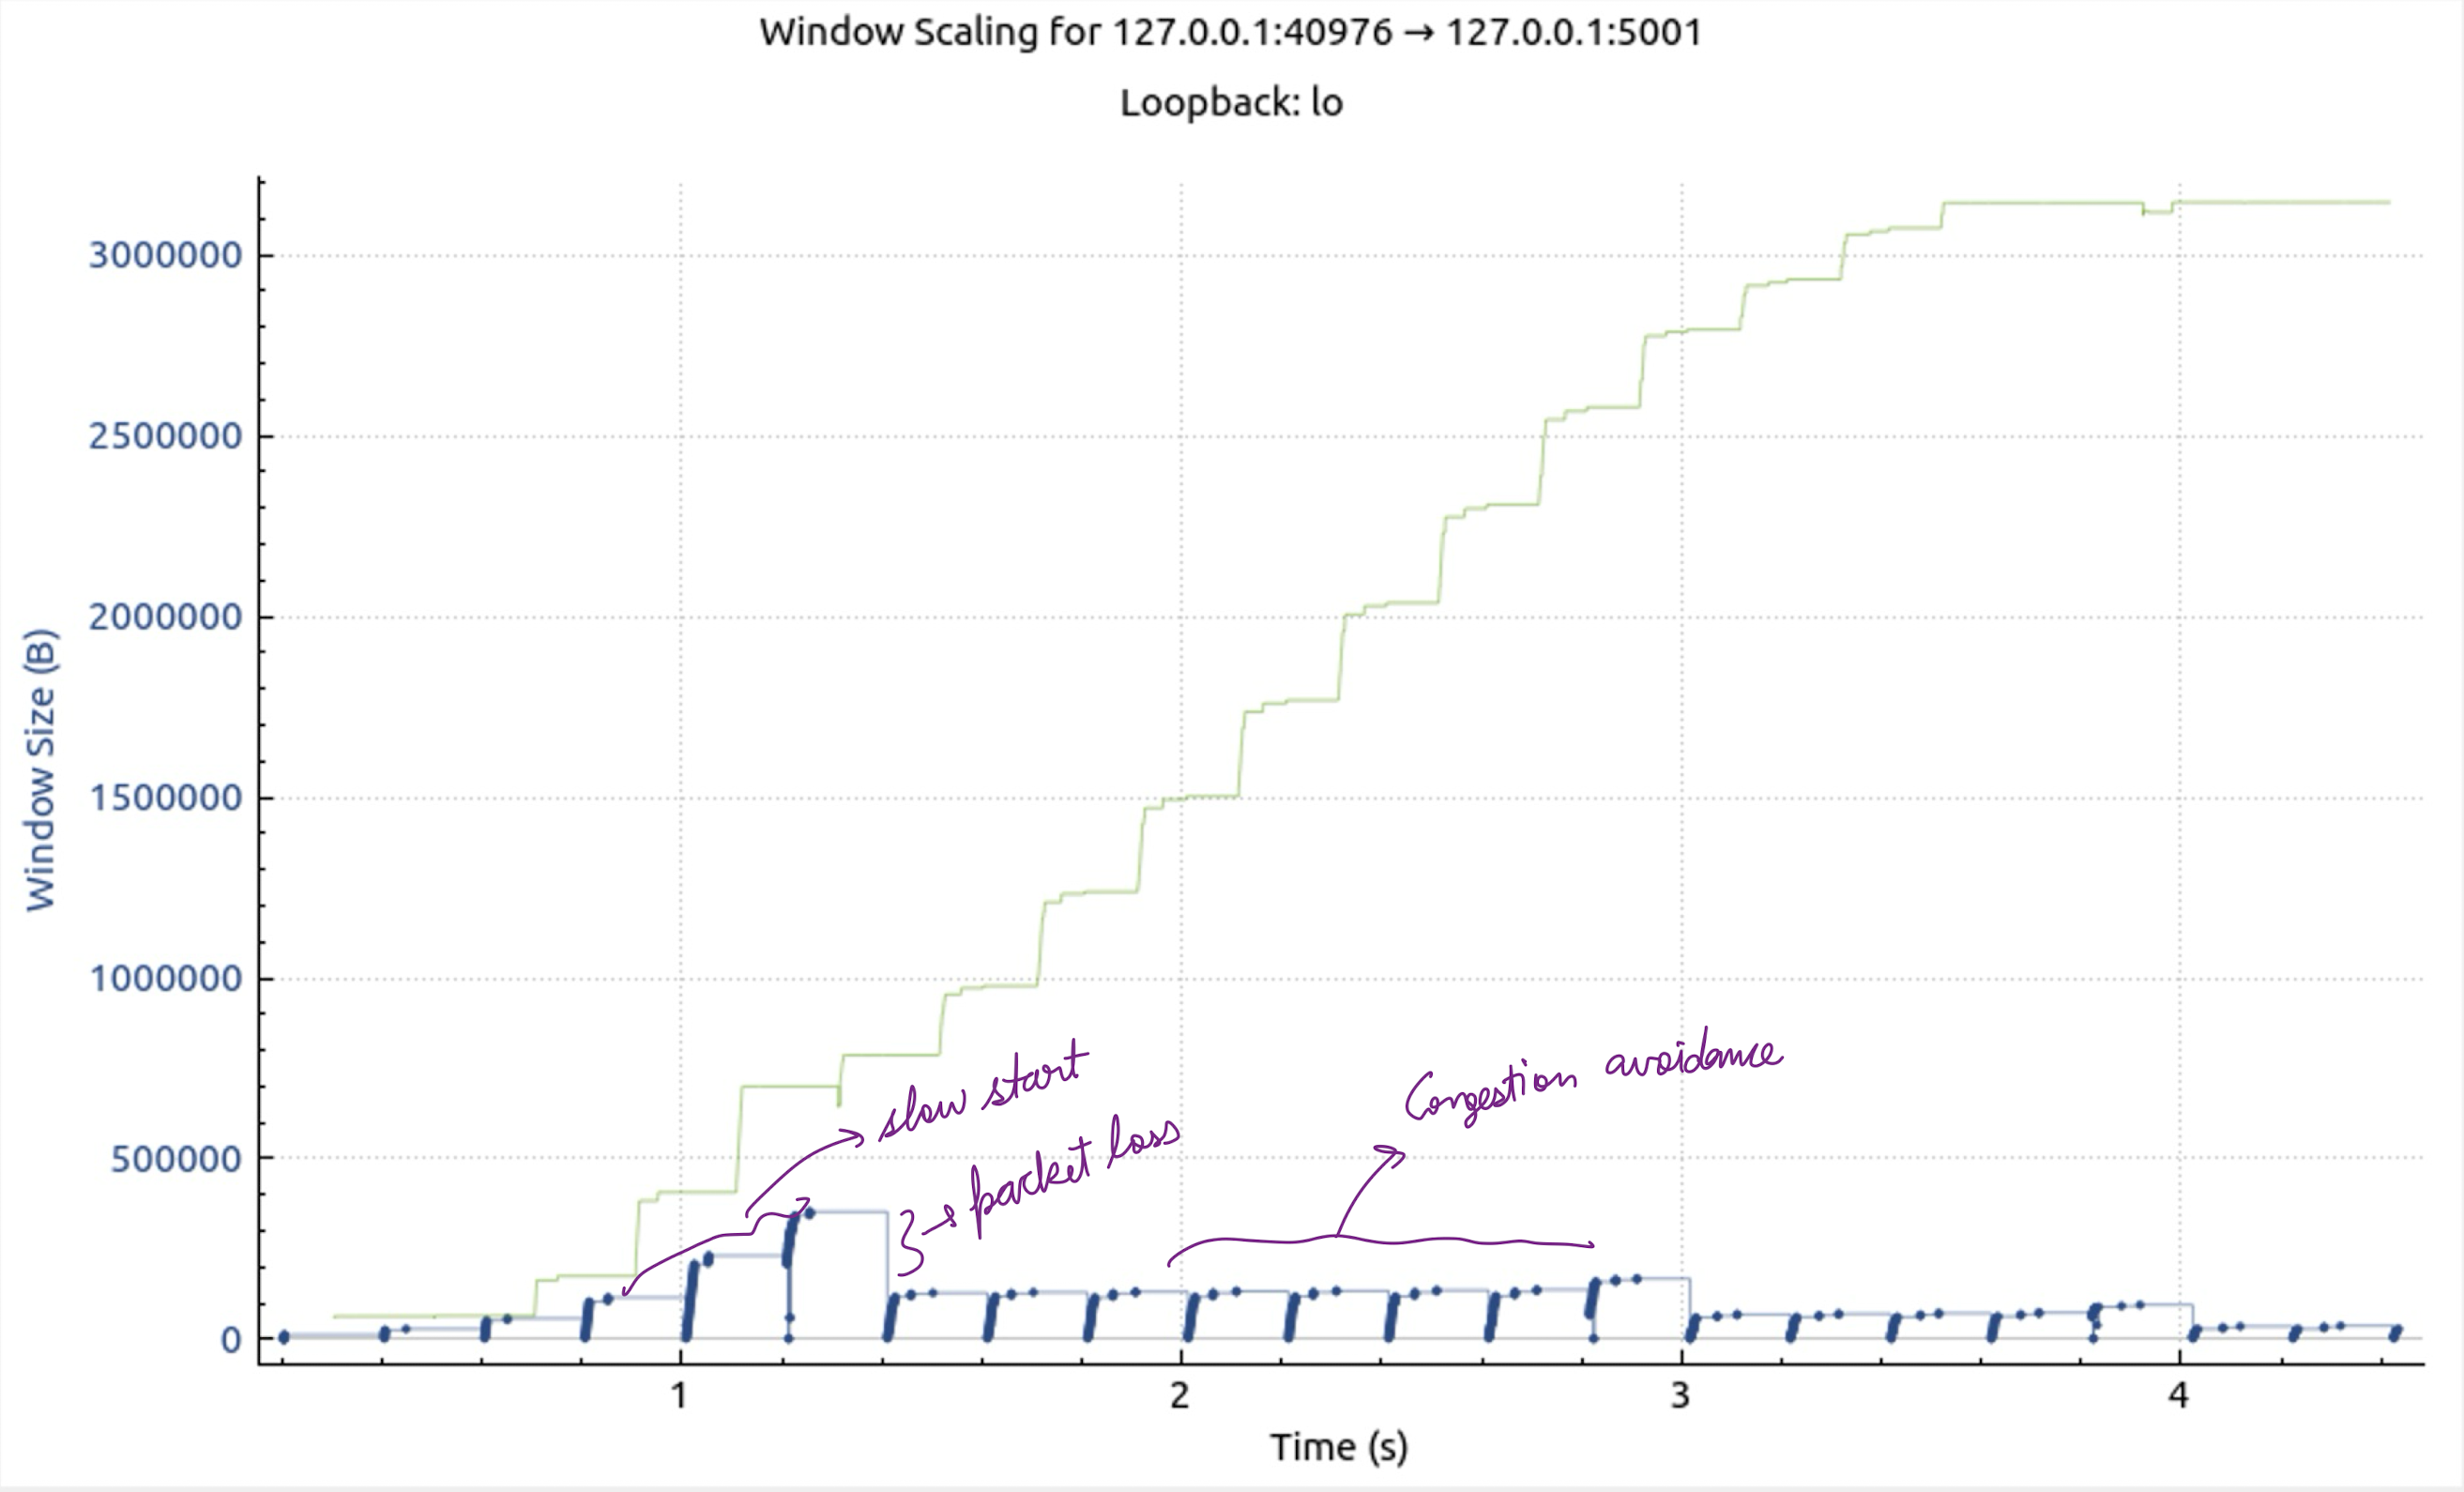
\includegraphics[width=0.8\textwidth]{reno-e2.png}
        \caption{Reno Window Scaling Graph for Delay=100ms and Loss=1\%}
    \end{figure}

    \begin{figure}[H]
        \centering
        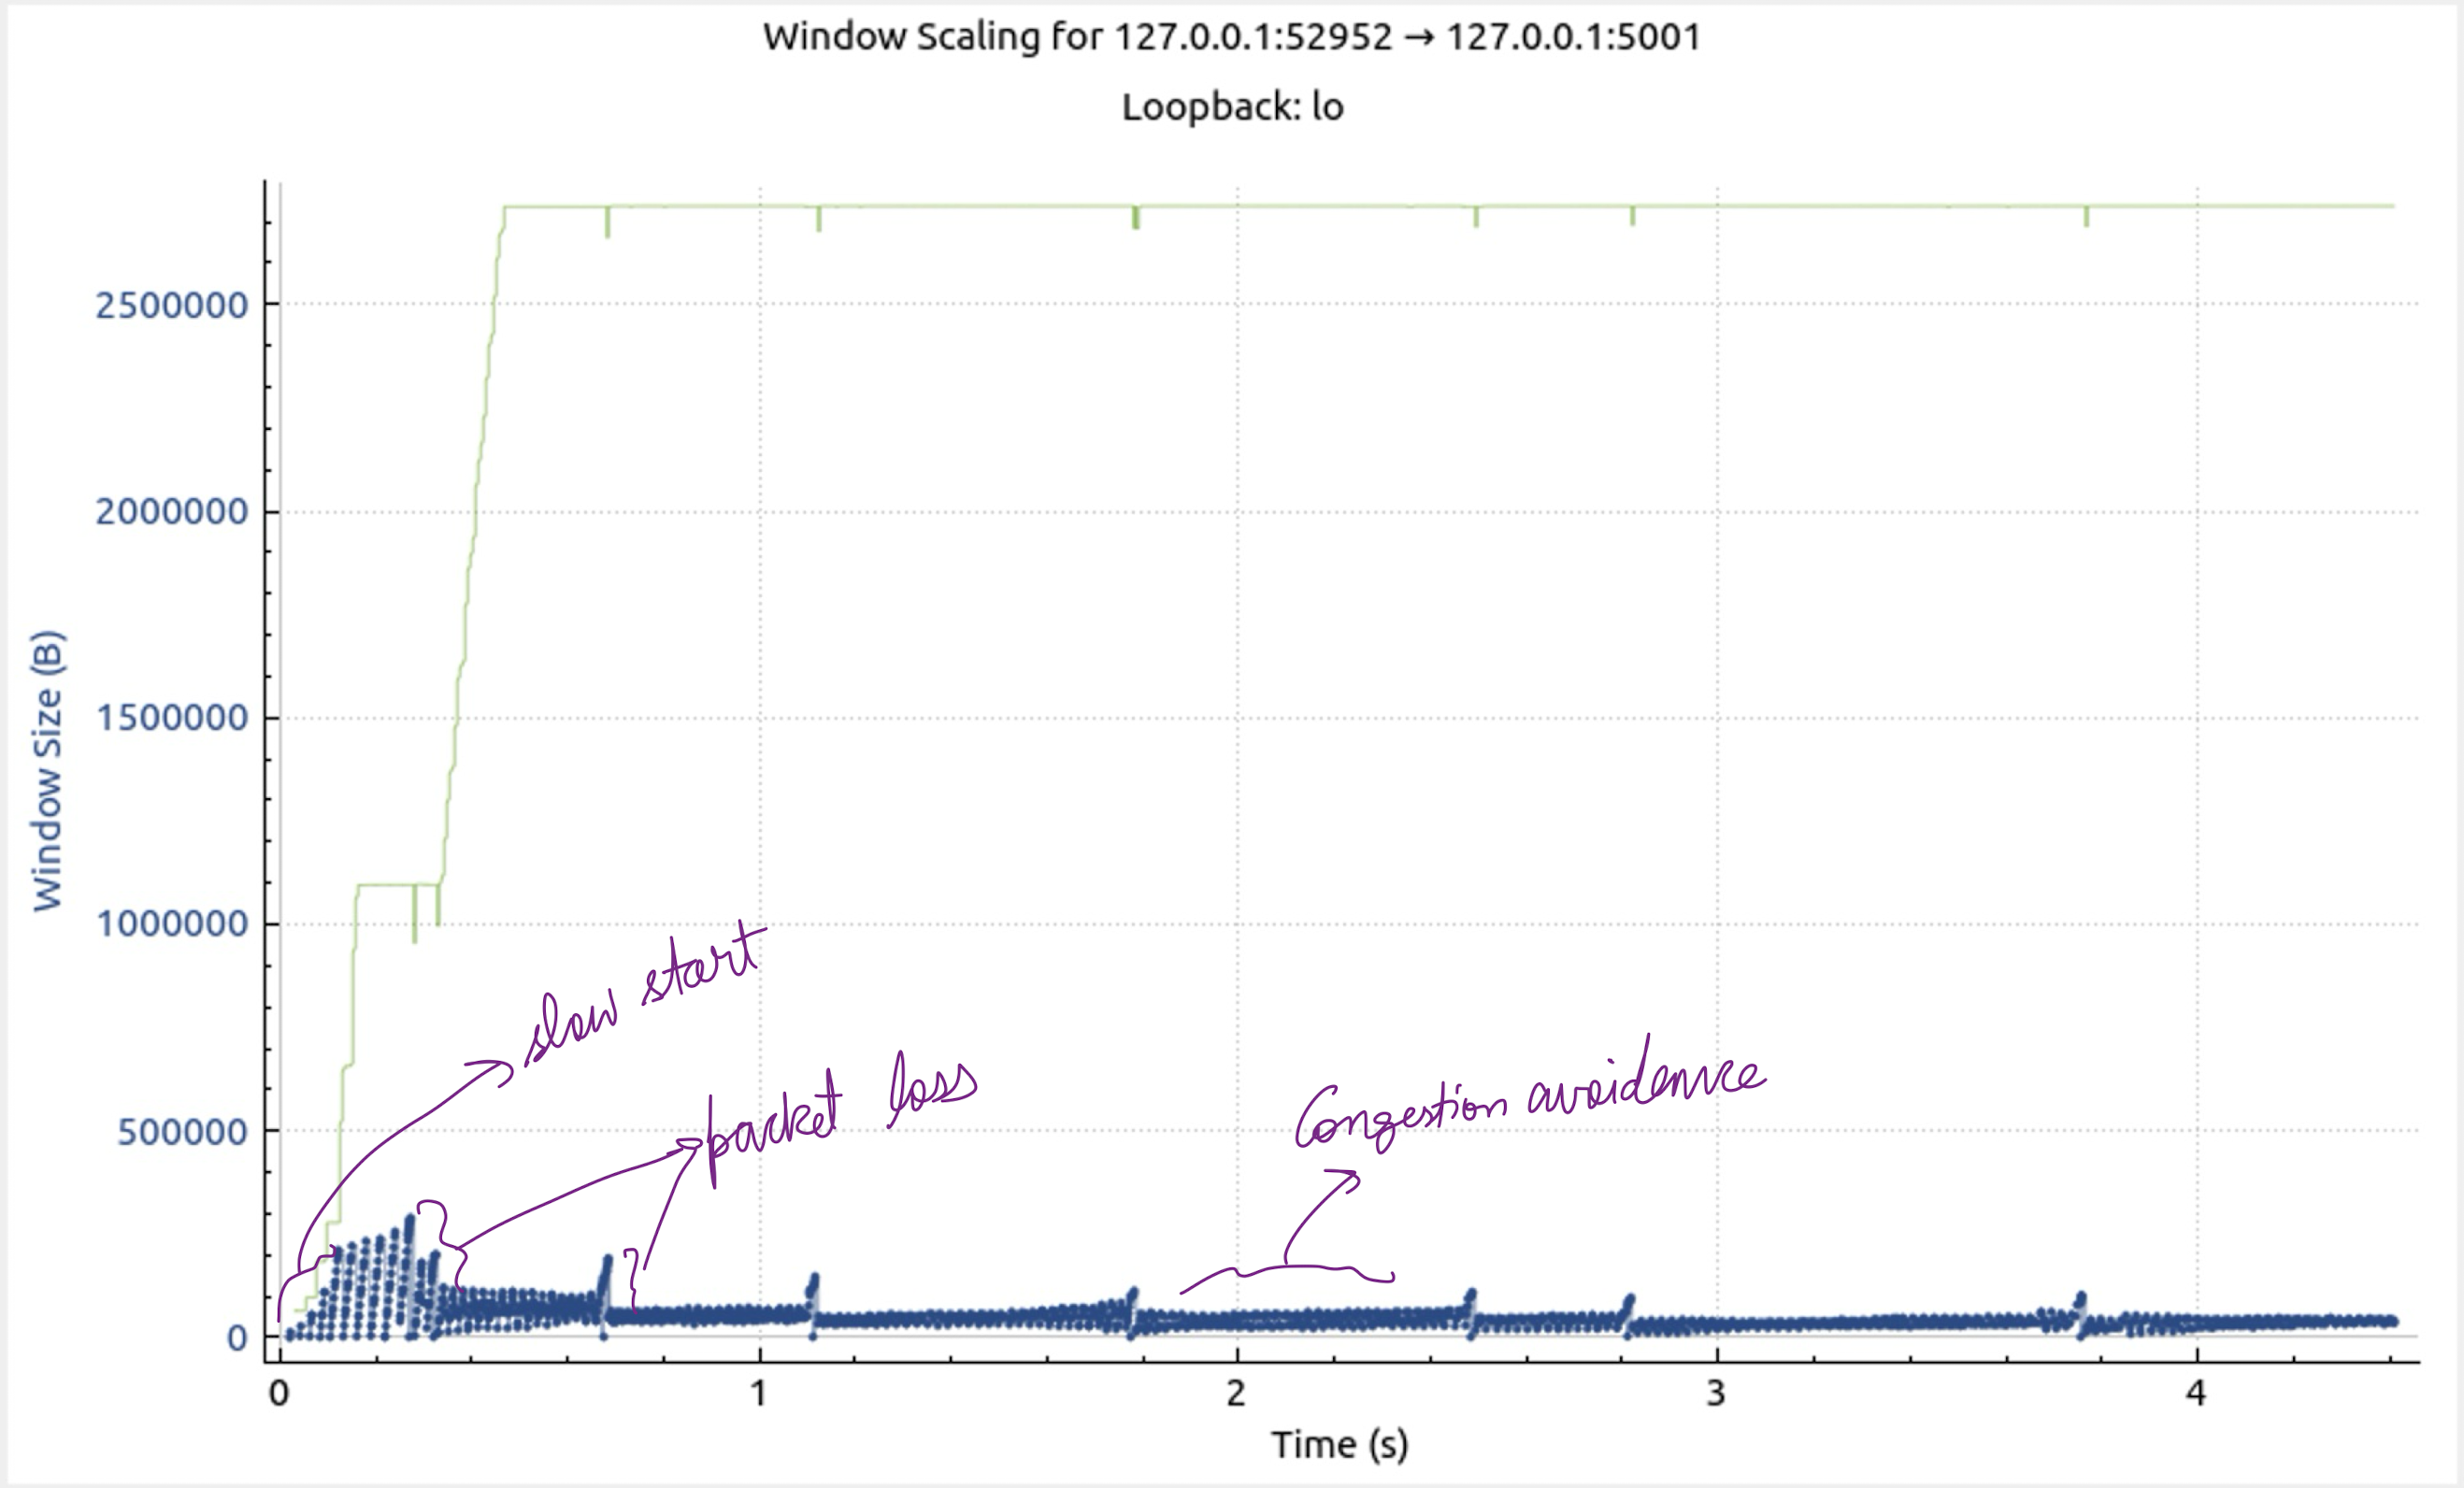
\includegraphics[width=0.8\textwidth]{cubic-e1.png}
        \caption{Cubic Window Scaling Graph for Delay=10ms and Loss=0.1\%}
    \end{figure}

    \begin{figure}[H]
        \centering
        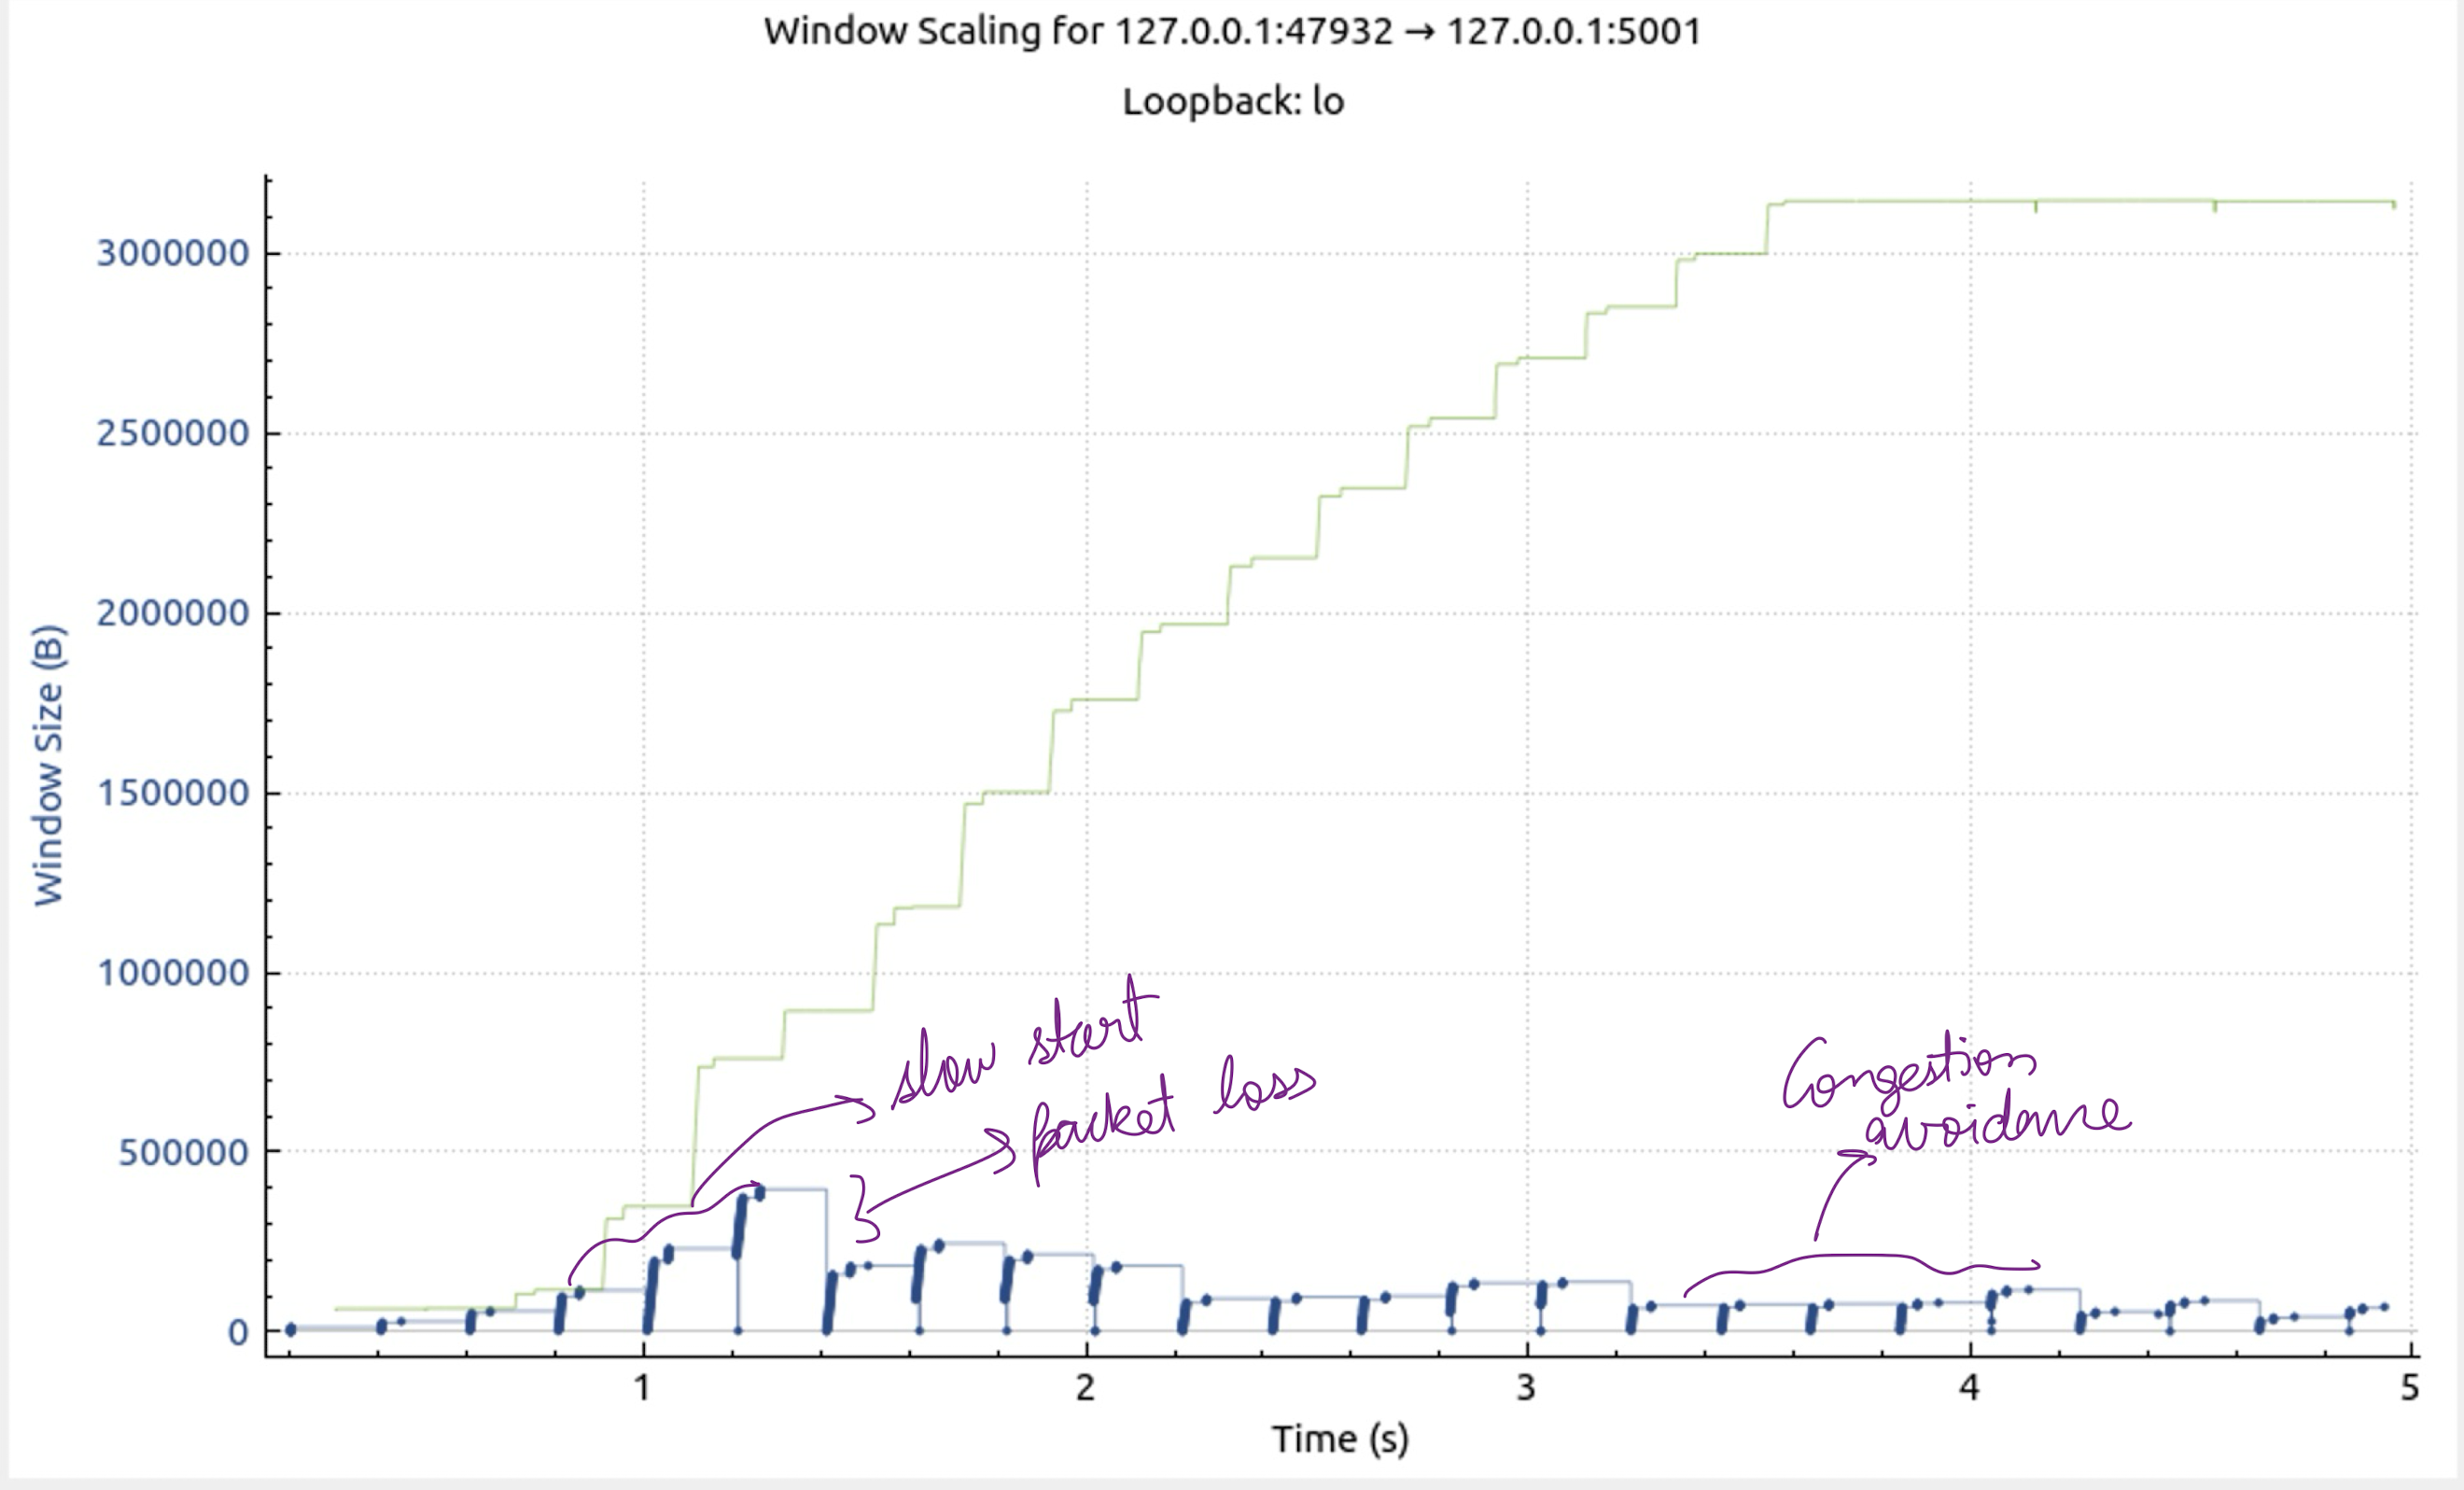
\includegraphics[width=0.8\textwidth]{cubic-e2.png}
        \caption{Cubic Window Scaling Graph for Delay=100ms and Loss=1\%}
    \end{figure}


    \begin{itemize}
        \item The plots in green are for window sizes, whereas the plots in blue are the unacked outstanding bytes (bytes in flight). 
        \item The annotations are shown in pink. 
        \item Locations where we see an exponential (sudden) increase in the window size correspond to slow start (present at the start or after a timeout).
        \item Similarly, locations where we see a sudden drop in the window size correspond to packet losses.
        \item Locations where we see a linear increase in the window size correspond to congestion avoidance.
        \item The window sizes are in general higher for cubic than for reno (specially after the initial section). This is because cubic is more aggressive in increasing the congestion window size.
    \end{itemize}
\end{solution}

\end{document}
